%-----------------------------------------------------------------------------------------
\clearpage
\section{Implementation}
%-----------------------------------------------------------------------------------------
In this section we describe how the project is implemented in detail. The subsystems executed are data reading, visualization rendering and the user options. Screen captures of the GUI are added to illustrate further information.

\subsection{Data Processing}

The main concept of data processing is to read text data from .txt files, calculate values need, and store them into Java Arraylist. At this stage, the greatest challenge is to keep the data being accessible and can be changed, as  the new data may be written over the old due to events in other class. Hence, after the original data is read and stored, it is retrieved and modified through  mutator methods \cite{Bob's coding convention}. In addtion to the flexibility, another difficulty at this stage is generating values for each term and store them appropriately. As discussed in the Project Features section, the aim of the software we designed is to present information about terms and provide an concordance view for each version. In this project, we calculate and sort frequencies of terms; compute colour values; computed locations of strings; instantiate Rectangle objects to represent data; create arrays to store translations.

Java.io, which enables for system input and output through data streams \cite{javadoc java.io}, is used in this project. It serves as a data buffer and reader in this project. The FileReader class, which extends the InputStreamReader class, can be used to read character files which by default are assumed to be an appropriate size. Since the volume of data in each document is not large, we instantiate a FileReader (object) to access each text file. The other data reading class adopted is the BufferedReader class. It is used to read text data from a character-input stream, and buffer the data to provide efficient reading of strings, arrays and lines \cite{javadoc7}. Java.util is another package imported in the DataReader class. To store and access data, the ArrayList, Hashtable, and Map classes from this package are used. In addition, classes such as JsonObject, JsonReader, and JsonArray in Javax.json package are used to read data from a Json file.

The main class that is responsible for reading the original data file is the DataReader class. This class analyses .txt files and generates a list of Version objects to parse all information needed in the software. Each Version object stores information of the concordance. For a more detailed description of the Version class and Item class, please see the Design section.

\subsection{Generating Concordances}

Concordances are the most basic visualisation in this project. They are designed to display the information of terms, and to help in comparing the terms between different translation versions.As shown in the Figure \ref{fig:condorVis}, the concordance visualisation involves several parts:
\begin{figure}[H]
	\centering	
	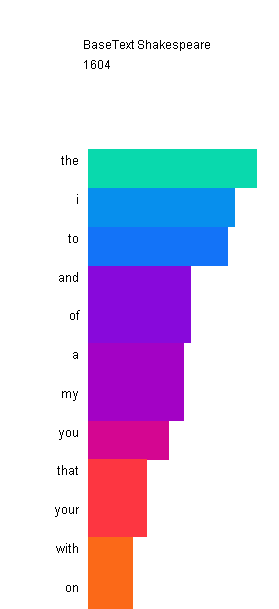
\includegraphics[width=9cm, height=15cm]{Figs/condordanceVis}\\[1ex]
	\caption{The Screen shot of one concordance in the visualisation}
	\label{fig:condorVis}
\end{figure} 

\begin{itemize}
	\item \textbf{String} is drawn to display the term, frequency, version author, publication year; 
	\item \textbf{Rectangle} is used to present the frequency. As the values are sorted in data processing phase, the width of rectangles are set according to these sorted values.
	\item \textbf{Colour} is used to present differences on frequency. Each colour represents a number of frequency, so there will be same colours in different terms.
\end{itemize}

The process in generating the concordance visualization goes through the following steps:
\begin{itemize}
	\item \textbf{} Obtain the string of each term from text source. This step is done in the DataReader class. Detailed illustration seeing Data Reading implementation section.
	\item \textbf{} Calculate the number of times, namely term frequency, of each term occurred in the text (See Data Reading implementation section).  	
	\item \textbf{} Calculate the rectangle width for each term using the frequency of term. The equation of the rectangle width calculating is show in Equation \eqref{rectWidth}:
	
	\begin{multline}\label{rectWidth}
	rectWidth=wordFrequency*unit*scaleValue
	\end{multline}
	
	Where unit is the width of each segment since the rectangle is composed of a number of segments. WordFrequency is the value deciding how many segments compose the rectangle, while scaleValue is the percentage value used to scale the rectangle, range from 10\% to 200\%.
	
	\item \textbf{}Calculate the location of the string and rectangle.The location, or point, is the start drawing point for the string and rectangle. It combined with two point value: point.X, and point.Y. The Equation \eqref{PointX}, \eqref{PointY} illustrate how we calculate these points in the software:
	
	\begin{multline}\label{PointX}
	point.x=versionNumber*versionDistance*scaleValue
	\end{multline}
	
	\begin{multline}\label{PointY}
	point.y= lineNumber*lineDistance*scaleValue
	\end{multline}
	
	Where versionNumber represents order number of the version. versionDistance performs the  distance between two neighbour versions. In addition, a scale value need to be multiplied so that the location of string and rectangle changes according to user preference.
	Similarly, the lineNumber is order number of the term while lineDistance represents the distance between two terms. 
	
	\item \textbf{}Calculate the value of colour. According to \cite{Jbum}, we use the equation as shown in Equation \eqref{Red}: 	
	\begin{multline}\label{Red}
	color = Math.sin(colorFrequency*wordFrequency + phase) * amplitude + center
	\end{multline}
	Where colorFrequency is a constant that controls how fast the wave oscillates. The wordFrequency is  variable used to display different colour according to word frequency. The phase is applied to change the alignment of the green or blue sine waves. The amplitude controls how high (or low) the wave goes. The center controls the center position of the wave.
	
	\item \textbf{}Paint the strings, blocks, and colours by invoking drawing methods in Graphic class. 
	
\end{itemize}

\subsection{Parallel View of Concordances}

Following the generation of concordance visualization, a parallel view of all concordances is created. As shown in Figure \ref{fig:parallelConcor}, all versions of concordances are represented on the panel. During this stage, lines will be drawn to connect same terms. The comparison stage is done in concordancePanel class. 

\begin{figure}[H]
	\centering	
	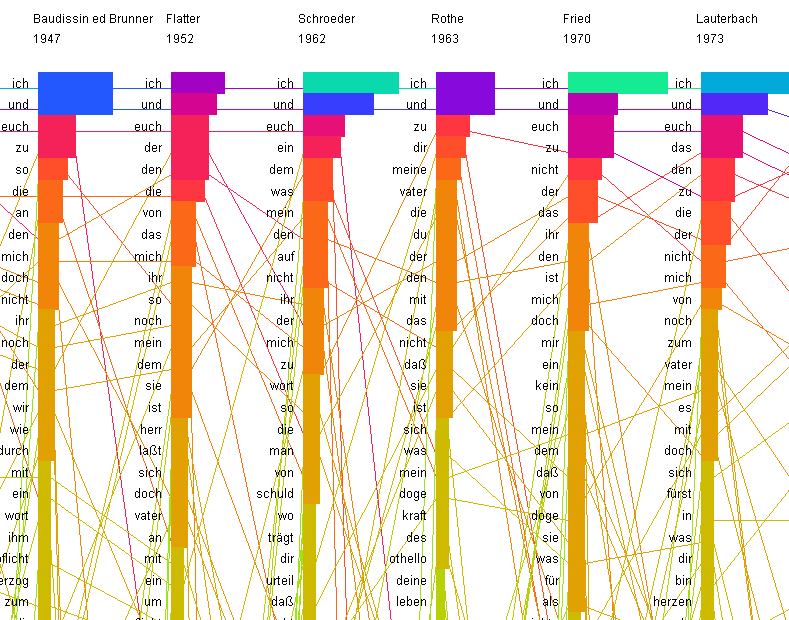
\includegraphics[width=13cm, height=8cm]{Figs/Parallel-Vis}\\[1ex]
	\caption{Parallel view of concordances}
	\label{fig:parallelConcor}
\end{figure} 


However, after this parallel visualization is being generated, an obvious problem appears: there is not enough space for all 16 concordances. So the solution is either to scale the panel, or to select several versions showing one time. We have done both, which are introduced in the following section. 

\subsection{Zooming}

Zooming in and out is a basic feature in the software which designed to provide two zooming options: one is for scaling the content of the visualisation, the other is for scaling the frame. In addition to these two scaling options, there are also scroll bars used to scroll the visualisation panel.

To implement these features, several steps as followed are gone through:
\begin{itemize}
	\item \textbf{} Generate the JSlider objects. This is carried out in the TranslationVisualization class. Figure \ref{fig:jSliders} displays the JSlider applied in the software.
	\begin{figure}[H]
		\centering	
		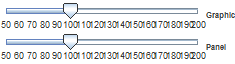
\includegraphics[width=9cm, height=3cm]{Figs/JSliders}\\[1ex]
		\caption{ Sliders applied to zoom in and out the graphic and panel}
		\label{fig:jSliders}
	\end{figure} 	
	\item \textbf{} Obtain scale values from JSlider object and pass them to DataReader class.
	\item \textbf{} Recalculated the data by invoking the calculating methods such as calculatePoint() and setRectWidth().
	\item \textbf{} Update the List<Version> object.
	\item \textbf{} Repaint graphics.
\end{itemize} 
 
During this process, the most difficult part is to recalculate all values of graphics: points, widths and heights for rectangles, and the distances between versions. To overcome this dilemma, two solutions are attempted:
At the first phase, scale() method in Graphics2D class is invoked. By applying this method, computer will calculate and repaint all the graphics using scale parameters passed in. However, when the project prompting to the Term Selecting phase (See Interactive Selection of Terms section below), a problem of obtaining mouse clicking location appears. Hence, the second phase of scaling visualisation comes out.  

At the second phase, scale values attained from JSlider objects are passed to DataReader class and applied in relevant formulas to calculate variables such as points, widths and heights of rectangles. See Equation \eqref{rectWidth}, \eqref{PointX}, and \eqref{PointY}. As shown in \ref{fig:jSliders}, 100 is set as the initial value for the slider, so that the visualisation shown when the visualisation generated at the first time is scaled as 100\%. Figure \ref{fig:zoomIn} and Figure \ref{fig:zoomOut} show the zooming results for the visualisation.

	\begin{figure}[H]
	\centering	
	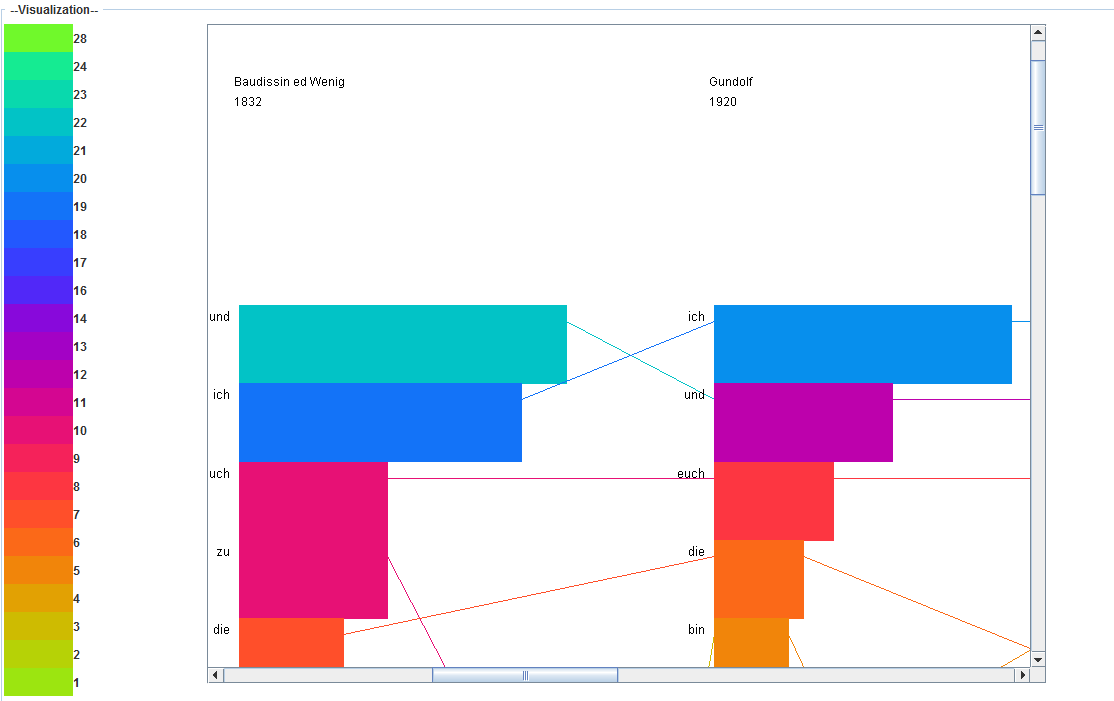
\includegraphics[width=9cm, height=3cm]{Figs/Zoom-In}\\[1ex]
	\caption{}
	\label{fig:zoomIn}
	\end{figure}

	\begin{figure}[H]
	\centering	
	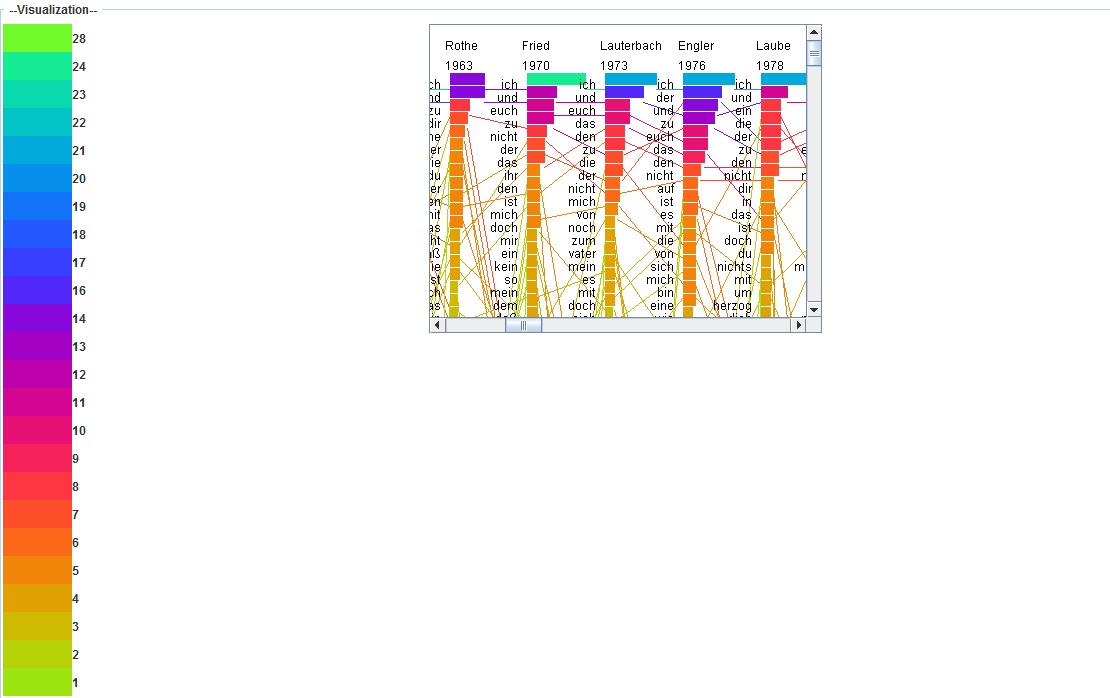
\includegraphics[width=9cm, height=3cm]{Figs/Zoom-Out}\\[1ex]
	\caption{}
	\label{fig:zoomOut}
	\end{figure}

\subsection{Text Labels On and Off}

When the scale values becoming smaller, the strings overlap. Hence a new desire appearing: hide strings on the visualisation. So that users can focus on the rectangles and colours only. 

To implement this feature, a JButton is generated on the panel firstly. Also, "Text On" is set as default label displayed on the button. Secondly, event listener is added to the button. When button is clicked, the label "Text On" on the button will be switched to "Text Off" label. In the meantime, a boolean value which set "true" as default will change to "false", then being given to ConcordancePanel class. In the third step, a boolean value preset when drawing strings of terms will be switched equals to the boolean value passed in. if it is "true", then draw the strings, if it is "false" then not invoke the drawString() method. At last, repaint the graphic. Figure \ref{fig:textOnOff} is a screen shot when we turn off the text.

\begin{figure}[H]
	\centering	
	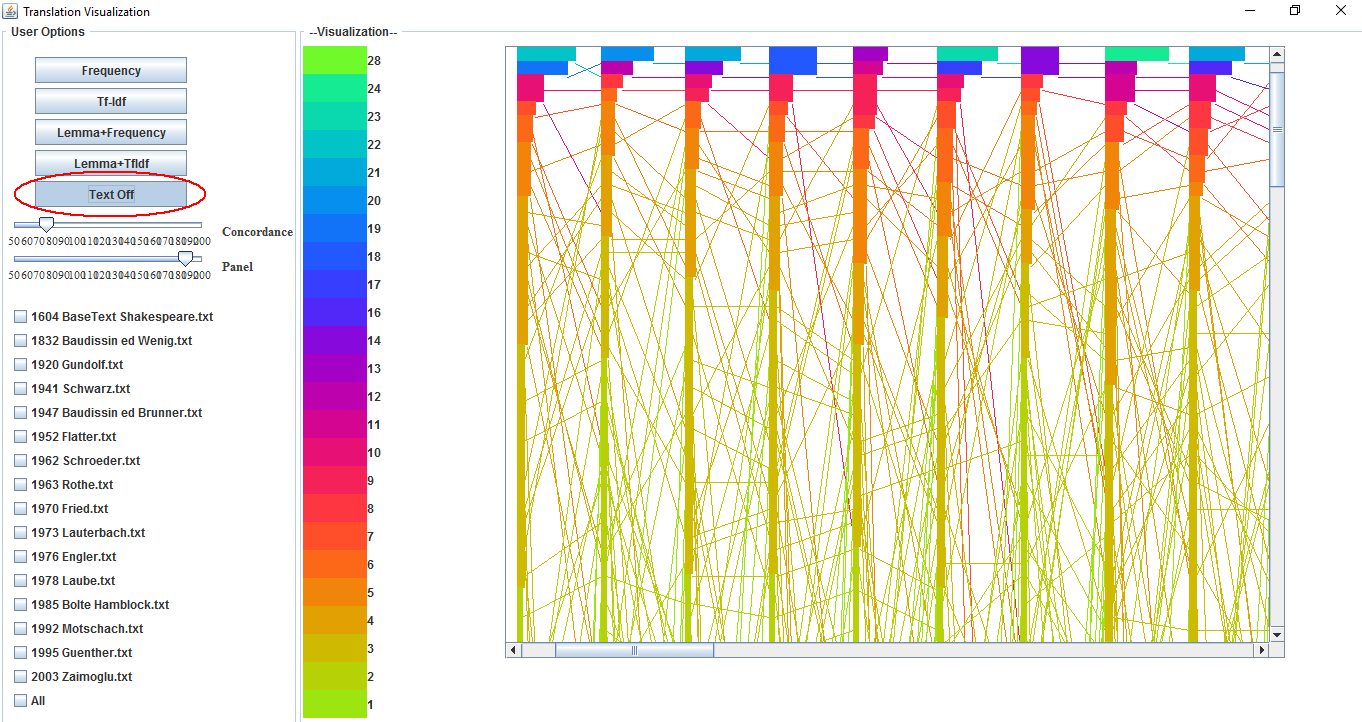
\includegraphics[width=18cm, height=12cm]{Figs/Text-On-Off}\\[1ex]
	\caption{}
	\label{fig:textOnOff}
\end{figure} 

\subsection{Adding, Subtracting, Selecting Items}

To render an user option feature for selecting several concordances displaying on the panel, a new class called VersionChoosenPanel is created. By interacting with this feature, not only can the user select which concordance to display in the visualization, but also the order of concordance displayed can be arranged. Figure
\ref{fig:versionChoosPanel} reveals the menu of version list can be selected. 
\begin{figure}[H]
	\centering	
	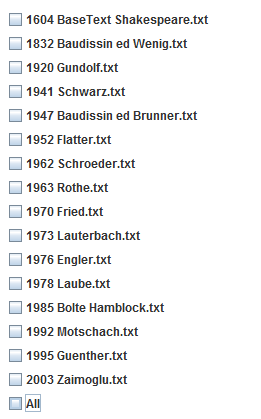
\includegraphics[width=6cm, height=10cm]{Figs/VersionChoosePanel}\\[1ex]
	\caption{The index of version selection}
	\label{fig:versionChoosPanel}
\end{figure} 

The generation of version selection feature goes through the following steps:
\begin{itemize}
	\item \textbf{} Generate a list of JCheckBox class to display the author name as the index. 
	\item \textbf{} Add event listener for each JCheckBox object. So that the action of selection can be generated as an Object class.
	\item \textbf{} Change the selecting status of the index. 
	\item \textbf{} Generate new list of Version objects according to the events passed from JCheckBox ActionListener. Every time the user select a name in the index, a new list of Version objects will be generated and passed to ConcordancePanel class. 
	\item \textbf{} Repaint the concordance visualisation. The ConcordancePanel will be repainted by invoking repaint() method.
	\item \textbf{} Add an option of "All" selection, which is responsible to display or hide all concordances as the original order.
\end{itemize}

Figure \ref{fig:versionChoosDemo}is a screen shot of selecting several versions of concordances to show on the visualisation. Further more, concordances are reordered on the visualisation, where the base text which supposed to be shown as the first version on the left, now being moved to the last one.

\begin{figure}[H]
	\centering	
	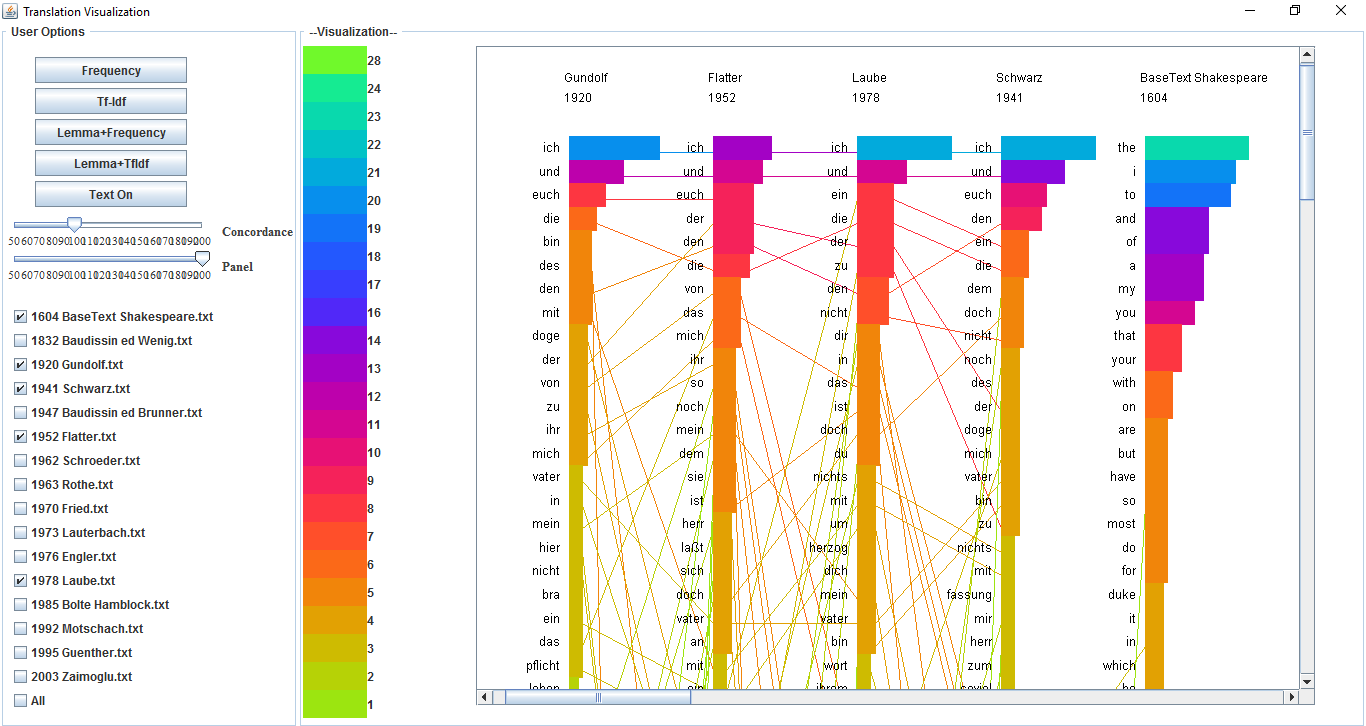
\includegraphics[width=18cm, height=10cm]{Figs/Version-Selecting-Demo}\\[1ex]
	\caption{The screen shot of version selecting feature}
	\label{fig:versionChoosDemo}
\end{figure} 

\subsection{Interaction and Selection of Terms}

On the ground that each concordance contains a large number of terms, highlight the term following users' options is desired. In order to provide an interactive features for terms, new feature are enable in the visualisation. Therefore a clear view of highlighting terms comes out. 

This features are achieved by put into effect following phases:
\begin{itemize}
	\item \textbf{} Obtain clicking point through getPoint() method in MouseEvent class.
	\item \textbf{} Calculate which item region the point belongs to. In this process, the regions of concordance and item are divided as illustrated in Figure \ref{fig:regionDivide}. As the value of each region can be achieved during data reading phase, the point passed from mouseClikcked() method can be used to identify which region the point belongs. Further more, the Item object of this block is singled out and returned.
	\begin{figure}[H]
		\centering	
		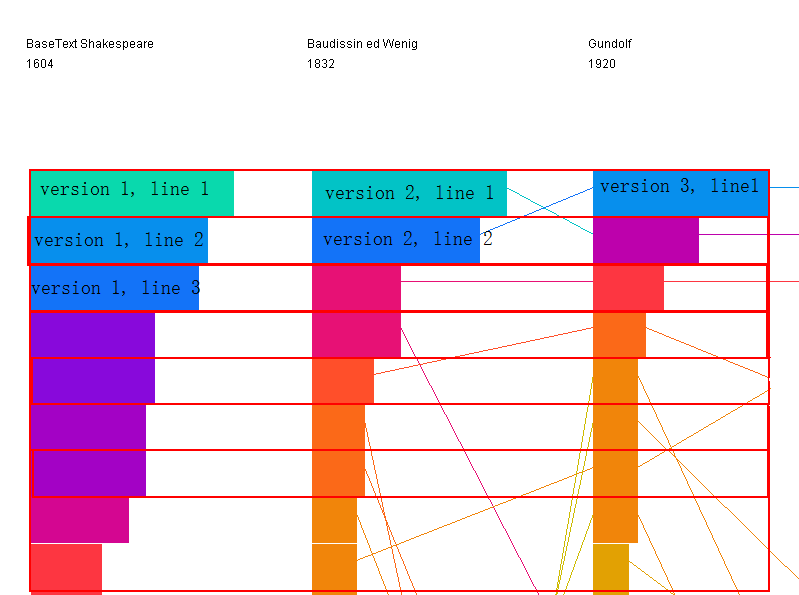
\includegraphics[width=6cm, height=10cm]{Figs/Region-Divide}\\[1ex]
		\caption{}
		\label{fig:regionDivide}
	\end{figure} 
	\item \textbf{} Identify the Item objects in other concordances sharing the same term. So that we get Item objects to be highlighted.
	\item \textbf{} Highlight the blocks of all singled out Item objects. In this step, lines are drawn to round the rectangles. 
	\item \textbf{} Make other blocks transparent. The transparency values of other rectangles are set as  semitransparent values by overwriting colour values of blocks.
	\item \textbf{} Overwritten the colour values of all lines to make sure lines connecting two highlighting items are highlighted as well, while other lines becoming semitransparent.
	\item \textbf{} Find out the translations of this term and highlight the blocks of them.	
\end{itemize}

As a result, by clicking one single rectangle in the panel, the rectangle is highlighted and rounded by line while the colour of other rectangles become transparent. In the mean time, lines connecting same terms become highlighted by setting other lines transparent. See Figure \ref{fig:highlightView}

\begin{figure}[H]
	\centering	
	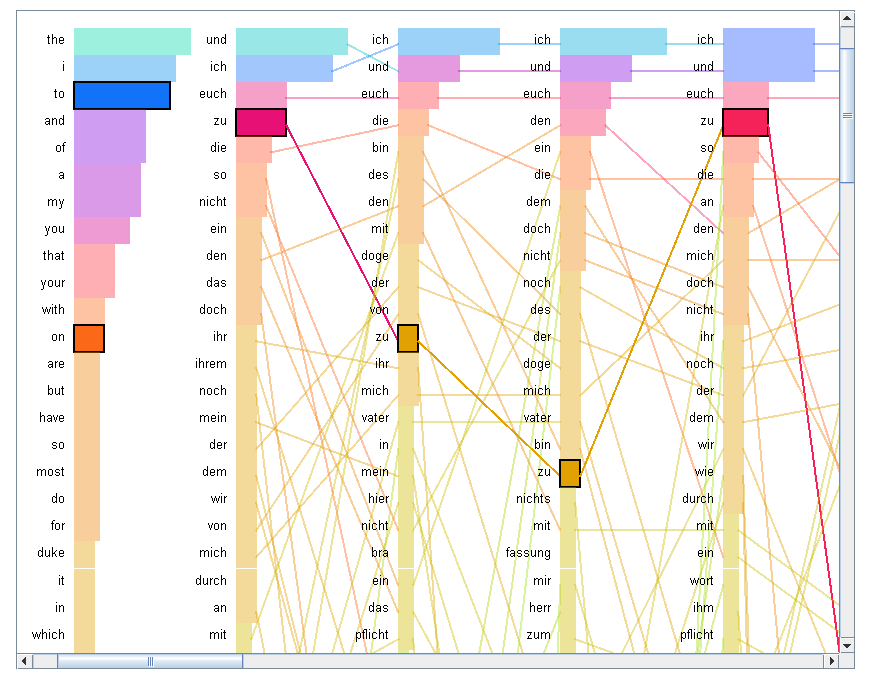
\includegraphics[width=16cm, height=9cm]{Figs/Highlight-Terms}\\[1ex]
	\caption{}
	\label{fig:highlightView}
\end{figure} 

\subsection{Colour Mapping}

Colour represents the occurrences of terms in each concordance. To demonstrate all colours in the visualisation, colour mapping is essential. In this project, we instantiate a ColorLegendPanel class to fulfill this feature. In addition, values of the frequency is displayed in the Colour Mapping view. Following is the process to implement this function: 
\begin{itemize}
	\item \textbf{} Achieve the colour value of each item from DataReader object. The detailed illustration of colour values can be retrieved in Data Reading chapter.
	\item \textbf{} Instantiate JLabel objects as the components representing colours.
	\item \textbf{} Add the JLabel objects to the panel.
	\item \textbf{} Display frequency values beside colour blocks.
\end{itemize}

The demo of Colour Mapping is shown in Figure \ref{fig:colourMapping}.
\begin{figure}[H]
	\centering	
	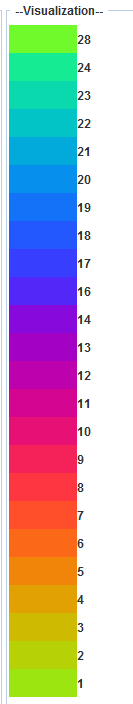
\includegraphics[width=4cm, height=15cm]{Figs/Color-Mapping}\\[1ex]
	\caption{}
	\label{fig:colourMapping}
\end{figure} 

\subsection{Interactive Color Legend}

Apart from displaying data, colour mapping can be served as interactive visualisation. In this project, we add an feature so that user can interact with the colour legend. If the user click a label of colour in the colour legend, all blocks of that colour in the concordance view will be highlighted. This function is performed by identifying all items possessing same frequency value. As illustrated in the Design chapter, an index of frequency values is generated in DataReader class. After data reading phase, we can access this list of frequency values through accessor method. By iterating all values in the list, the items are identified and returned to ConcordancePanel class. Then the list of Version objects are overwritten and the panel is repainted.

As a result, by clicking one colour block in colour legend, all items sharing same frequency, or colour, are highlighted using same methods of highlighting described in Interaction and Selection of Terms chapter. Figure \ref{fig:interactiveColourMapping} serves as a demo to illustrate this feature.
\begin{figure}[H]
	\centering	
	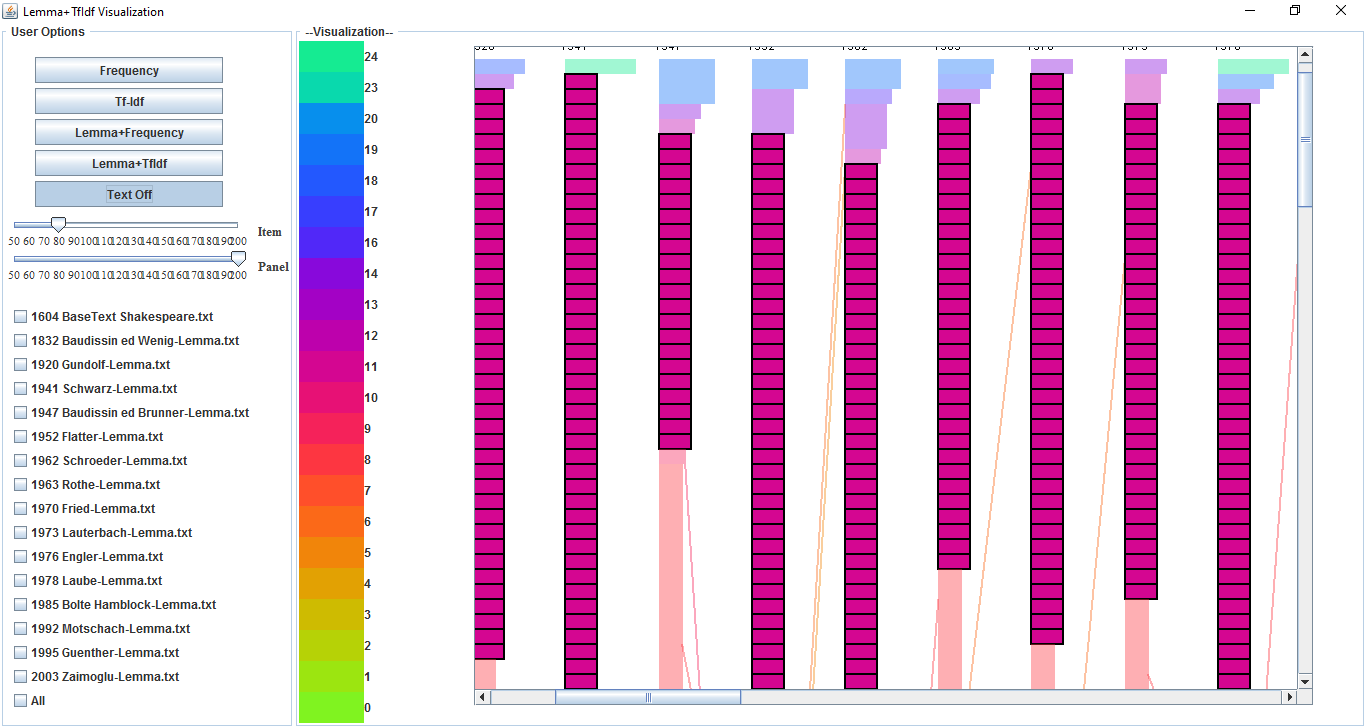
\includegraphics[width=16cm, height=12cm]{Figs/Colour-Legend-Interation}\\[1ex]
	\caption{}
	\label{fig:interactiveColourMapping}
\end{figure} 

\subsection{Lemmatisation}

The lemma visualisation a significant feature in this project. Lemma is a linguistic term which described as the dictionary form of a word. Take the English word 'decide' for example: 'decide' is the lemma for 'decided', 'decides', 'deciding'. Accordingly, lemmatisation is the process to obtain the lemma for each word. To achieve the effect of lemma view, several steps is necessary:
\begin{itemize}
	\item \textbf{} Obtain the German lemma corpus which contains an index of lemmas and words.
	\item \textbf{} Compare the words in our German translation corpus with the words in the German lemma corpus, and find the lemma for each term in our corpus.
	\item \textbf{} Store all the lemmas being found and generate a new lemma index.
	\item \textbf{} Apply the lemmas into visualisation.
\end{itemize}
For this project, an inevitable dilemma is the limited resources of German lemma corpus. As illustrated in Data Characteristics chapter, there is no relevant German lemma corpus in this project when we start this project. Also, German, as an affected language, is difficult to lemmatise. It is more challenging to acquire this kind of corpus from other sources. During this process, we attempted two solutions: Treetagger and DeReWo, which will be explained in following sections.

\subsubsection{TreeTagger}

As introduced in Technology Choices chapter, the TreeTagger is a tool for annotating text data and lemma information. Figure \ref{fig:treeTaggerUI} shows the Interface of TreeTagger. During applying this tool in the lemmatizing task of the project, we found this tool has following advantages:

\begin{figure}[H]
	\centering	
	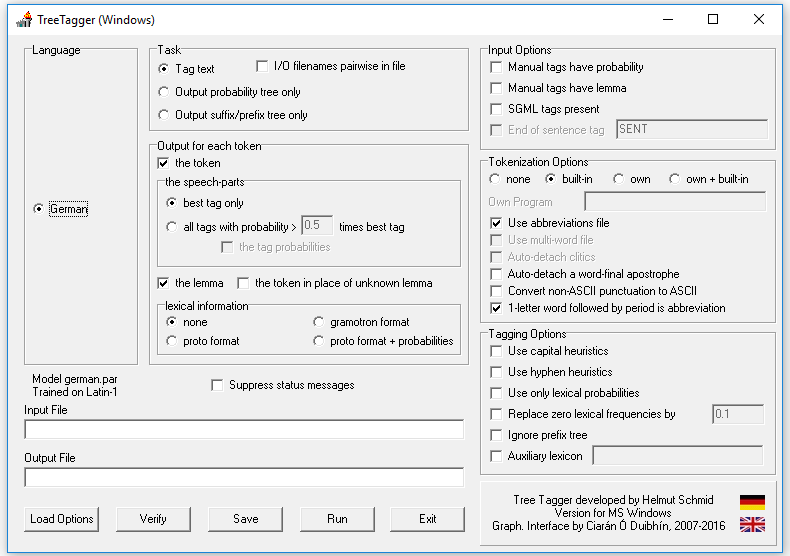
\includegraphics[width=16cm, height=12cm]{Figs/TreeTaggerInterface}\\[1ex]
	\caption{}
	\label{fig:treeTaggerUI}
\end{figure} 

\begin{itemize}
	\item \textbf{} The software is easy to obtain. Without any redundant procedures such as registration, the tool can be downloaded directly from the website \url{http://www.cis.uni-muenchen.de/~schmid/tools/TreeTagger/}.
	\item \textbf{} The user interface of the tool is clear and easy to use.
	\item \textbf{} The concept in using software is to upload a .txt file, create a .txt file to store results, and lemmatise the data.	
\end{itemize}

However, there are also some problems we encountered:
\begin{itemize}
	\item \textbf{} The format of the text file must be encoded in Latin-1, while the text file we have is encoded in UTF-8. Therefore, some German terms with special characters cannot be recognised by the tool.
	\item \textbf{} From the results we achieved, the tool cannot recognise words with capital letters. 
	\item \textbf{} The tool cannot be used to lemmatise a group of files at one time, which is not appropriate for project which needs to process large data sets. 	
\end{itemize}

We connected an domain expert, Dr. Tom Cheesman form the Mordern Language Center of Swansea University, to evaluate the results of the lemmatisation for TreeTagger. Appendix {?} is the file of sample lemma we sent to Dr. Cheesman with the comments he sent back. Due to the low accuracy of the results for the data in this project, this solution is given up in the end.

\subsubsection{DeReWo}

DeReWo is a project done by Institut Fur Deutsche Sprache. This project aims at developing methods to create frequncy-based ranking lists of lemma based on random virtual corpora. In the DeReWo website \url{http://www1.ids-mannheim.de/direktion/kl/projekte/methoden/derewo.html?L=1}, there are some downloadable resources of German lemma, including 'DeReKo-2014-II-MainArchive-STT.100000.freq', which is a file storing top 100,000 German words, lemmas and POS. The format of this document is .freq, which can be edit in Visual Studio Code. It also can be read from Java directly. Using this corpus, we successrully obtain all the lemmas for each term in the \emph{Othello} corpus for this project.

There are several phases of using DeReWo to generate lemma visualisation:
\begin{itemize}
	\item \textbf{} Read text file from \emph{Othello} corpus.	
	\item \textbf{} Read German lemma corpus file.
	\item \textbf{} Search for the lemma of each term.
	\item \textbf{} Store the lemma in a new text file. In this step, we create 15 .txt files for all German translation. Meanwhile, order of the lemma is kept as the same with their original text. For each version of \emph{Othello} translation, the two files (\emph{Othello} source file and lemma file) are served as an index for words and lemmas.
	\item \textbf{} Replace all terms with according lemmas and visualise the new results.
\end{itemize}	

Figure \ref{fig:lemmaView} shows the outcome of the lemma visualisation. 

\begin{figure}[H]
	\centering	
	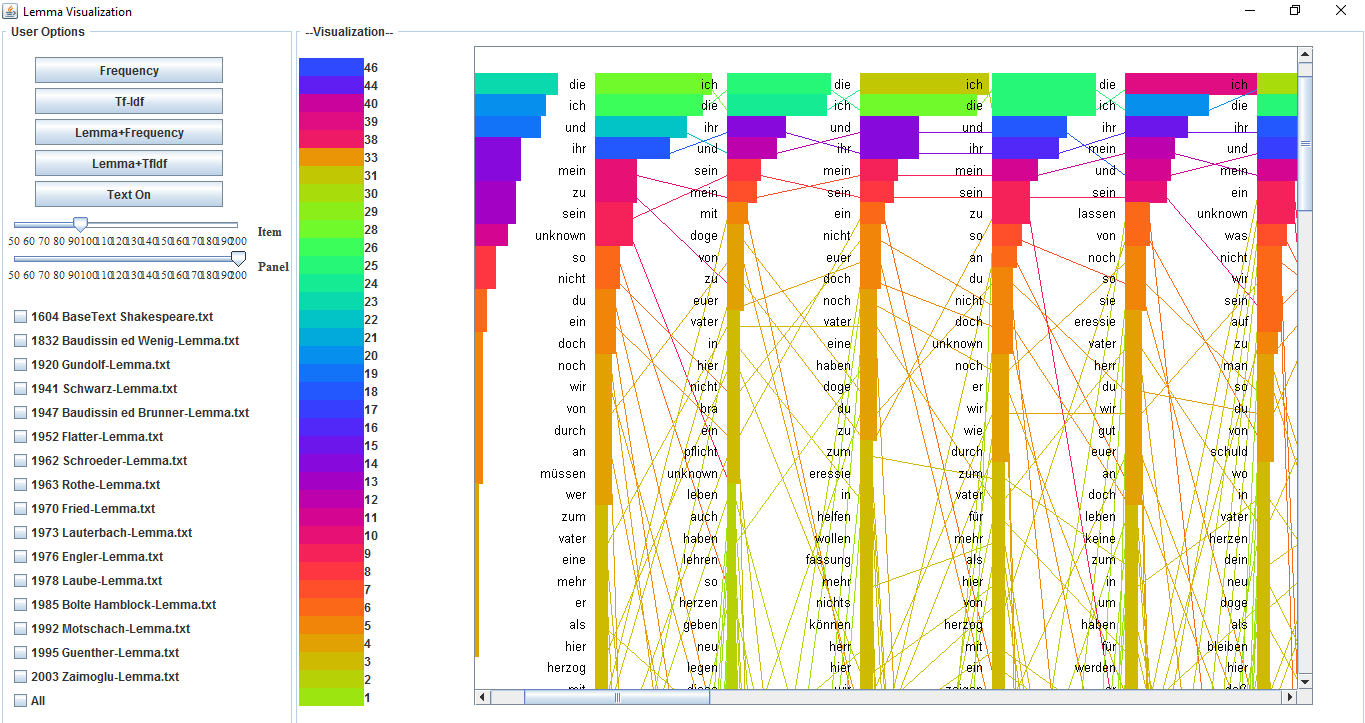
\includegraphics[width=16cm, height=12cm]{Figs/LemmaView}\\[1ex]
	\caption{}
	\label{fig:lemmaView}
\end{figure} 

\subsection{Tf-Idf}

Tf-Idf visualisation is an important feature in this project. As explained in Design chapter, the Tf-Idf value represents weightings of words, which also means we can get rid of unimportant words, namely stopping words. Therefore, the visualisation provided will be more helpful for researchers to study the varieties of translation. To fulfill this function, the most challenging step is to apply the formula of the Tf-Idf into the codes. Equation \ref{Tf-Idf} is used in this project to calculate the Tf-Idf value for each term \cite{Asking Mohammad about the equation referance}. The TfIdfCalculator class is created to process the Tf-Idf values.

The Tf-Idf visualisation generation process goes through the following steps:

\begin{itemize}
\item \textbf{} Calculate term frequency value. This step is done in the data reading stage. The Tf value hence can be achieved from DataReader object.
\item \textbf{} Calculate Idf value. As shown in Equation \ref{Tf-Idf},
\item \textbf{} Replace the frequency with Tf-Idf value.
\item \textbf{} Visulise according to new results.
\end{itemize} 

There are two visualisation generated using Tf-Idf value: one is to visualise data using Tf-Idf value and original words, as shown in Figure \ref{fig:tfIdfView}; the other is to visualise using Tf-Idf value together with lemma data which is displayed in Figure \ref{fig:tfIdfLemma}.

\begin{figure}[H]
	\centering	
	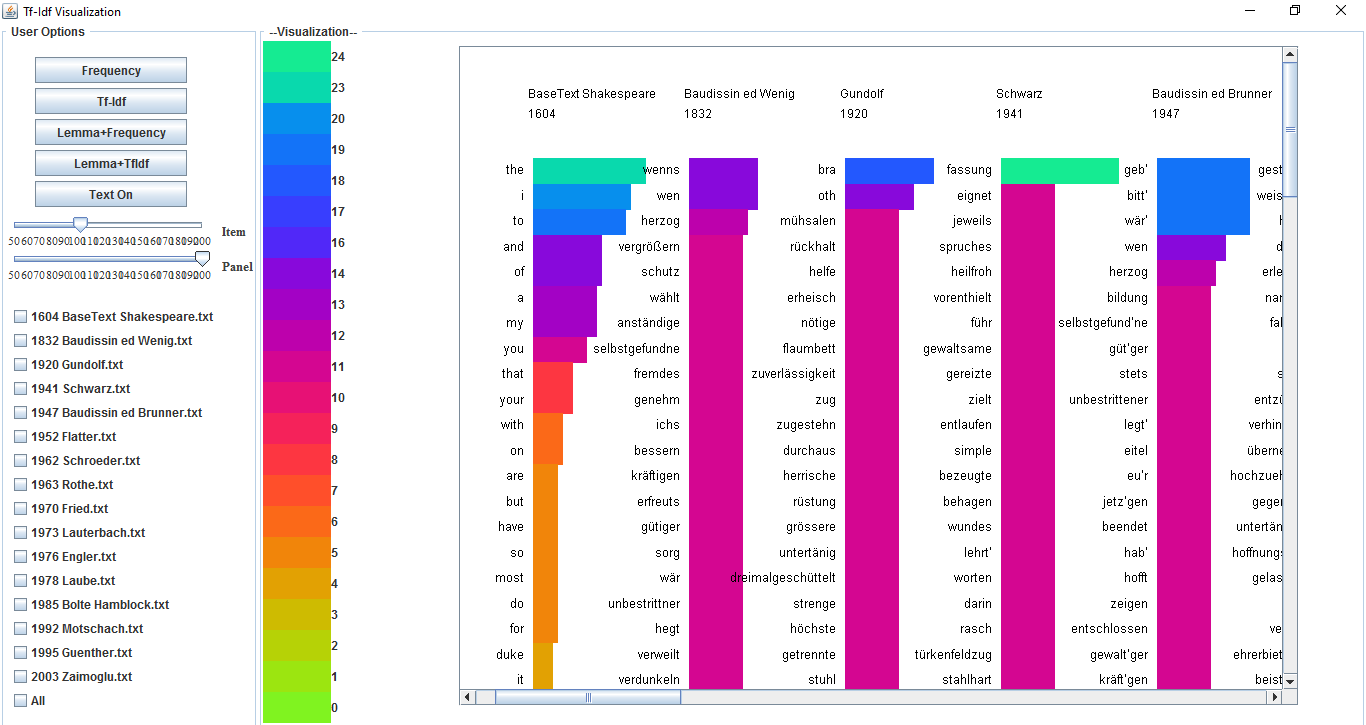
\includegraphics[width=16cm, height=12cm]{Figs/Tf-Idf}\\[1ex]
	\caption{}
	\label{fig:tfIdfView}
\end{figure} 
\begin{figure}[H]
	\centering	
	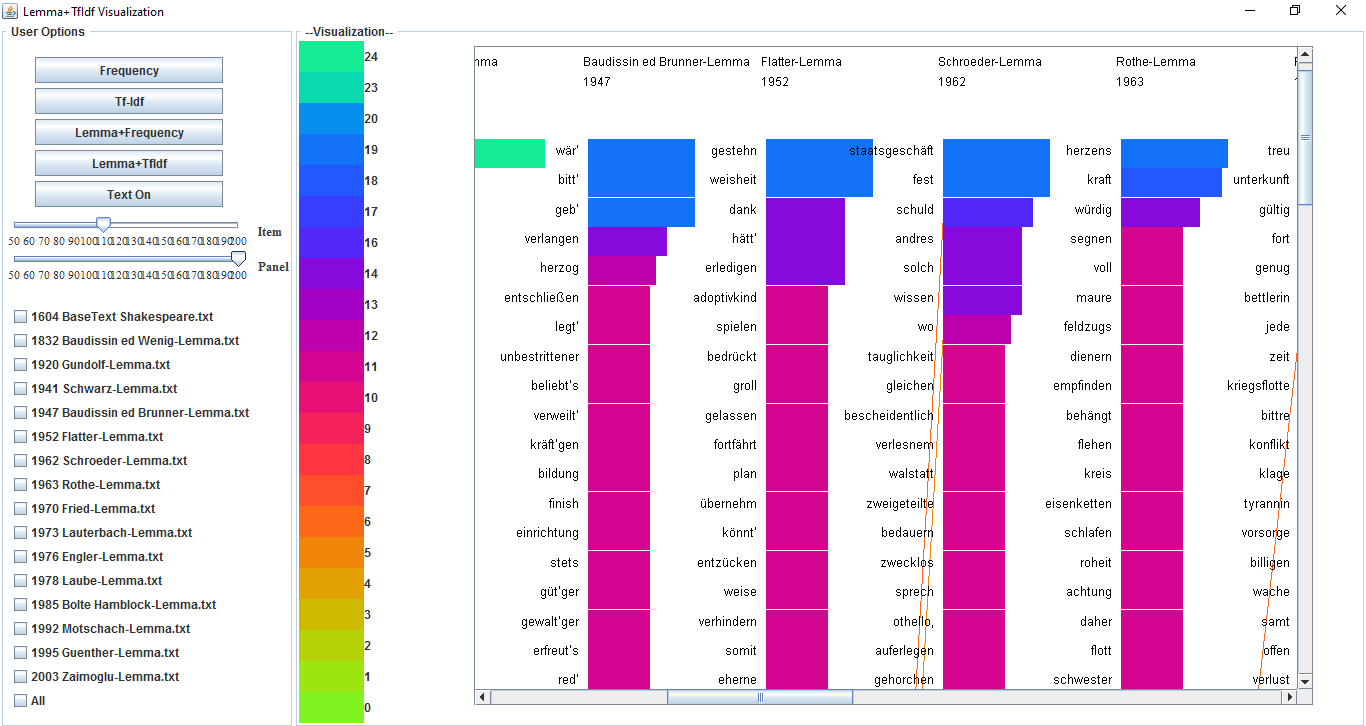
\includegraphics[width=16cm, height=12cm]{Figs/Lemma-TfIdf}\\[1ex]
	\caption{}
	\label{fig:tfIdfLemma}
\end{figure} 


